% Options for packages loaded elsewhere
% Options for packages loaded elsewhere
\PassOptionsToPackage{unicode}{hyperref}
\PassOptionsToPackage{hyphens}{url}
\PassOptionsToPackage{dvipsnames,svgnames,x11names}{xcolor}
%
\documentclass[
  letterpaper,
  DIV=11,
  numbers=noendperiod]{scrartcl}
\usepackage{xcolor}
\usepackage{amsmath,amssymb}
\setcounter{secnumdepth}{5}
\usepackage{iftex}
\ifPDFTeX
  \usepackage[T1]{fontenc}
  \usepackage[utf8]{inputenc}
  \usepackage{textcomp} % provide euro and other symbols
\else % if luatex or xetex
  \usepackage{unicode-math} % this also loads fontspec
  \defaultfontfeatures{Scale=MatchLowercase}
  \defaultfontfeatures[\rmfamily]{Ligatures=TeX,Scale=1}
\fi
\usepackage{lmodern}
\ifPDFTeX\else
  % xetex/luatex font selection
\fi
% Use upquote if available, for straight quotes in verbatim environments
\IfFileExists{upquote.sty}{\usepackage{upquote}}{}
\IfFileExists{microtype.sty}{% use microtype if available
  \usepackage[]{microtype}
  \UseMicrotypeSet[protrusion]{basicmath} % disable protrusion for tt fonts
}{}
\makeatletter
\@ifundefined{KOMAClassName}{% if non-KOMA class
  \IfFileExists{parskip.sty}{%
    \usepackage{parskip}
  }{% else
    \setlength{\parindent}{0pt}
    \setlength{\parskip}{6pt plus 2pt minus 1pt}}
}{% if KOMA class
  \KOMAoptions{parskip=half}}
\makeatother
% Make \paragraph and \subparagraph free-standing
\makeatletter
\ifx\paragraph\undefined\else
  \let\oldparagraph\paragraph
  \renewcommand{\paragraph}{
    \@ifstar
      \xxxParagraphStar
      \xxxParagraphNoStar
  }
  \newcommand{\xxxParagraphStar}[1]{\oldparagraph*{#1}\mbox{}}
  \newcommand{\xxxParagraphNoStar}[1]{\oldparagraph{#1}\mbox{}}
\fi
\ifx\subparagraph\undefined\else
  \let\oldsubparagraph\subparagraph
  \renewcommand{\subparagraph}{
    \@ifstar
      \xxxSubParagraphStar
      \xxxSubParagraphNoStar
  }
  \newcommand{\xxxSubParagraphStar}[1]{\oldsubparagraph*{#1}\mbox{}}
  \newcommand{\xxxSubParagraphNoStar}[1]{\oldsubparagraph{#1}\mbox{}}
\fi
\makeatother

\usepackage{color}
\usepackage{fancyvrb}
\newcommand{\VerbBar}{|}
\newcommand{\VERB}{\Verb[commandchars=\\\{\}]}
\DefineVerbatimEnvironment{Highlighting}{Verbatim}{commandchars=\\\{\}}
% Add ',fontsize=\small' for more characters per line
\usepackage{framed}
\definecolor{shadecolor}{RGB}{241,243,245}
\newenvironment{Shaded}{\begin{snugshade}}{\end{snugshade}}
\newcommand{\AlertTok}[1]{\textcolor[rgb]{0.68,0.00,0.00}{#1}}
\newcommand{\AnnotationTok}[1]{\textcolor[rgb]{0.37,0.37,0.37}{#1}}
\newcommand{\AttributeTok}[1]{\textcolor[rgb]{0.40,0.45,0.13}{#1}}
\newcommand{\BaseNTok}[1]{\textcolor[rgb]{0.68,0.00,0.00}{#1}}
\newcommand{\BuiltInTok}[1]{\textcolor[rgb]{0.00,0.23,0.31}{#1}}
\newcommand{\CharTok}[1]{\textcolor[rgb]{0.13,0.47,0.30}{#1}}
\newcommand{\CommentTok}[1]{\textcolor[rgb]{0.37,0.37,0.37}{#1}}
\newcommand{\CommentVarTok}[1]{\textcolor[rgb]{0.37,0.37,0.37}{\textit{#1}}}
\newcommand{\ConstantTok}[1]{\textcolor[rgb]{0.56,0.35,0.01}{#1}}
\newcommand{\ControlFlowTok}[1]{\textcolor[rgb]{0.00,0.23,0.31}{\textbf{#1}}}
\newcommand{\DataTypeTok}[1]{\textcolor[rgb]{0.68,0.00,0.00}{#1}}
\newcommand{\DecValTok}[1]{\textcolor[rgb]{0.68,0.00,0.00}{#1}}
\newcommand{\DocumentationTok}[1]{\textcolor[rgb]{0.37,0.37,0.37}{\textit{#1}}}
\newcommand{\ErrorTok}[1]{\textcolor[rgb]{0.68,0.00,0.00}{#1}}
\newcommand{\ExtensionTok}[1]{\textcolor[rgb]{0.00,0.23,0.31}{#1}}
\newcommand{\FloatTok}[1]{\textcolor[rgb]{0.68,0.00,0.00}{#1}}
\newcommand{\FunctionTok}[1]{\textcolor[rgb]{0.28,0.35,0.67}{#1}}
\newcommand{\ImportTok}[1]{\textcolor[rgb]{0.00,0.46,0.62}{#1}}
\newcommand{\InformationTok}[1]{\textcolor[rgb]{0.37,0.37,0.37}{#1}}
\newcommand{\KeywordTok}[1]{\textcolor[rgb]{0.00,0.23,0.31}{\textbf{#1}}}
\newcommand{\NormalTok}[1]{\textcolor[rgb]{0.00,0.23,0.31}{#1}}
\newcommand{\OperatorTok}[1]{\textcolor[rgb]{0.37,0.37,0.37}{#1}}
\newcommand{\OtherTok}[1]{\textcolor[rgb]{0.00,0.23,0.31}{#1}}
\newcommand{\PreprocessorTok}[1]{\textcolor[rgb]{0.68,0.00,0.00}{#1}}
\newcommand{\RegionMarkerTok}[1]{\textcolor[rgb]{0.00,0.23,0.31}{#1}}
\newcommand{\SpecialCharTok}[1]{\textcolor[rgb]{0.37,0.37,0.37}{#1}}
\newcommand{\SpecialStringTok}[1]{\textcolor[rgb]{0.13,0.47,0.30}{#1}}
\newcommand{\StringTok}[1]{\textcolor[rgb]{0.13,0.47,0.30}{#1}}
\newcommand{\VariableTok}[1]{\textcolor[rgb]{0.07,0.07,0.07}{#1}}
\newcommand{\VerbatimStringTok}[1]{\textcolor[rgb]{0.13,0.47,0.30}{#1}}
\newcommand{\WarningTok}[1]{\textcolor[rgb]{0.37,0.37,0.37}{\textit{#1}}}

\usepackage{longtable,booktabs,array}
\newcounter{none} % for unnumbered tables
\usepackage{calc} % for calculating minipage widths
% Correct order of tables after \paragraph or \subparagraph
\usepackage{etoolbox}
\makeatletter
\patchcmd\longtable{\par}{\if@noskipsec\mbox{}\fi\par}{}{}
\makeatother
% Allow footnotes in longtable head/foot
\IfFileExists{footnotehyper.sty}{\usepackage{footnotehyper}}{\usepackage{footnote}}
\makesavenoteenv{longtable}
\usepackage{graphicx}
\makeatletter
\newsavebox\pandoc@box
\newcommand*\pandocbounded[1]{% scales image to fit in text height/width
  \sbox\pandoc@box{#1}%
  \Gscale@div\@tempa{\textheight}{\dimexpr\ht\pandoc@box+\dp\pandoc@box\relax}%
  \Gscale@div\@tempb{\linewidth}{\wd\pandoc@box}%
  \ifdim\@tempb\p@<\@tempa\p@\let\@tempa\@tempb\fi% select the smaller of both
  \ifdim\@tempa\p@<\p@\scalebox{\@tempa}{\usebox\pandoc@box}%
  \else\usebox{\pandoc@box}%
  \fi%
}
% Set default figure placement to htbp
\def\fps@figure{htbp}
\makeatother


% definitions for citeproc citations
\NewDocumentCommand\citeproctext{}{}
\NewDocumentCommand\citeproc{mm}{%
  \begingroup\def\citeproctext{#2}\cite{#1}\endgroup}
\makeatletter
 % allow citations to break across lines
 \let\@cite@ofmt\@firstofone
 % avoid brackets around text for \cite:
 \def\@biblabel#1{}
 \def\@cite#1#2{{#1\if@tempswa , #2\fi}}
\makeatother
\newlength{\cslhangindent}
\setlength{\cslhangindent}{1.5em}
\newlength{\csllabelwidth}
\setlength{\csllabelwidth}{3em}
\newenvironment{CSLReferences}[2] % #1 hanging-indent, #2 entry-spacing
 {\begin{list}{}{%
  \setlength{\itemindent}{0pt}
  \setlength{\leftmargin}{0pt}
  \setlength{\parsep}{0pt}
  % turn on hanging indent if param 1 is 1
  \ifodd #1
   \setlength{\leftmargin}{\cslhangindent}
   \setlength{\itemindent}{-1\cslhangindent}
  \fi
  % set entry spacing
  \setlength{\itemsep}{#2\baselineskip}}}
 {\end{list}}
\usepackage{calc}
\newcommand{\CSLBlock}[1]{\hfill\break\parbox[t]{\linewidth}{\strut\ignorespaces#1\strut}}
\newcommand{\CSLLeftMargin}[1]{\parbox[t]{\csllabelwidth}{\strut#1\strut}}
\newcommand{\CSLRightInline}[1]{\parbox[t]{\linewidth - \csllabelwidth}{\strut#1\strut}}
\newcommand{\CSLIndent}[1]{\hspace{\cslhangindent}#1}



\setlength{\emergencystretch}{3em} % prevent overfull lines

\providecommand{\tightlist}{%
  \setlength{\itemsep}{0pt}\setlength{\parskip}{0pt}}



 


\KOMAoption{captions}{tableheading}
\makeatletter
\@ifpackageloaded{caption}{}{\usepackage{caption}}
\AtBeginDocument{%
\ifdefined\contentsname
  \renewcommand*\contentsname{Table of contents}
\else
  \newcommand\contentsname{Table of contents}
\fi
\ifdefined\listfigurename
  \renewcommand*\listfigurename{List of Figures}
\else
  \newcommand\listfigurename{List of Figures}
\fi
\ifdefined\listtablename
  \renewcommand*\listtablename{List of Tables}
\else
  \newcommand\listtablename{List of Tables}
\fi
\ifdefined\figurename
  \renewcommand*\figurename{Figure}
\else
  \newcommand\figurename{Figure}
\fi
\ifdefined\tablename
  \renewcommand*\tablename{Table}
\else
  \newcommand\tablename{Table}
\fi
}
\@ifpackageloaded{float}{}{\usepackage{float}}
\floatstyle{ruled}
\@ifundefined{c@chapter}{\newfloat{codelisting}{h}{lop}}{\newfloat{codelisting}{h}{lop}[chapter]}
\floatname{codelisting}{Listing}
\newcommand*\listoflistings{\listof{codelisting}{List of Listings}}
\makeatother
\makeatletter
\makeatother
\makeatletter
\@ifpackageloaded{caption}{}{\usepackage{caption}}
\@ifpackageloaded{subcaption}{}{\usepackage{subcaption}}
\makeatother
\usepackage{bookmark}
\IfFileExists{xurl.sty}{\usepackage{xurl}}{} % add URL line breaks if available
\urlstyle{same}
\hypersetup{
  pdftitle={Predicting Flight Delays in the United States: A Machine Learning Analysis of Weather{,} Network Effects{,} and Operational Factors},
  colorlinks=true,
  linkcolor={blue},
  filecolor={Maroon},
  citecolor={Blue},
  urlcolor={Blue},
  pdfcreator={LaTeX via pandoc}}


\title{Predicting Flight Delays in the United States: A Machine Learning
Analysis of Weather, Network Effects, and Operational Factors}
\author{Jonathan Wilson \and Karan Nindra \and Irena Austin \and Val
Sokolow}
\date{2026-03-13}
\begin{document}
\maketitle


\section{Abstract}\label{abstract}

Flight delays remain one of the most persistent operational challenges
in modern aviation, affecting airline efficiency, passenger
satisfaction, and the broader transportation network. In this study, we
examine flight delays within the United States using machine learning,
exploratory data analysis, and engineered operational features.

Using Bureau of Transportation Statistics (BTS) flight records enriched
with weather and temporal features, we construct predictors related to
schedule timing, prior aircraft movement, weather conditions, and
airport-level activity. We evaluate multiple supervised and unsupervised
learning approaches and even some neural networks using LSTMs.

Our findings suggest that delay behavior is shaped by a combination of
operational and environmental effects, especially upstream aircraft
delay propagation, airport congestion patterns, and weather-related
variables. Tree-based (with extreme gradient boosting) approaches and
penalized regression provide the most stable predictive performance,
while simpler baseline models remain valuable for interpretation.

\begin{center}\rule{0.5\linewidth}{0.5pt}\end{center}

\section{Introduction \& Background}\label{introduction-background}

\subsection{Motivation}\label{motivation}

Flight delays represent one of the most visible operational challenges
in modern aviation. A single disruption can ripple across aircraft
rotations, crews, passengers, and airports, creating cascading effects
throughout the network.

Understanding the causes of delay propagation is critical for improving
airline efficiency and passenger reliability.

\subsection{Related Works}\label{related-works}

\begin{itemize}
\tightlist
\item
  Add at least 3
\end{itemize}

\subsection{Research Questions}\label{research-questions}

This study seeks to answer the following questions:

\begin{enumerate}
\def\labelenumi{\arabic{enumi}.}
\tightlist
\item
  Which operational and weather variables most strongly predict flight
  delays?
\item
  How strongly do delays propagate from prior flights?
\item
  Which machine learning models best classify delayed flights?
\end{enumerate}

\subsection{What This Research
Contributes}\label{what-this-research-contributes}

This study contributes a route-focused machine learning framework for
airline delay analysis. By combining exploratory analysis, feature
engineering, classification modeling, and model comparison, we provide a
systematic approach for identifying the drivers of flight delays.

\section{Data and Methods}\label{data-and-methods}

\subsection{Data Sources \& Pipeline}\label{data-sources-pipeline}

\subsubsection{Data Pipeline}\label{data-pipeline}

The pipeline integrates three independent data streams --- Bureau of
Transportation Statistics (BTS) on-time performance records, NOAA Global
Surface Hourly weather observations, and airport reference dimensions
--- into a single analytical dataset suitable for delay prediction
modelling. Figure~\ref{fig-pipeline} provides a schematic overview of
each stage. The sections below describe each stage in turn.

\begin{figure}

\centering{

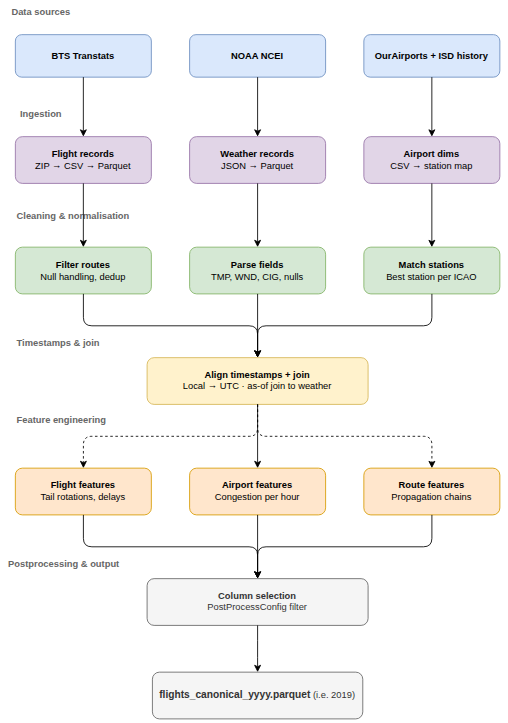
\includegraphics[width=1\linewidth,height=\textheight,keepaspectratio,alt={A flowchart showing seven stages of the flight delay pipeline: data sources, ingestion, cleaning and normalisation, timestamp alignment and join, feature engineering, postprocessing, and output.}]{images/common_site/data-pipeline.png}

}

\caption{\label{fig-pipeline}Overview of the flight delay data pipeline,
from raw data sources through ingestion, cleaning, temporal alignment,
feature engineering, and final output.}

\end{figure}%

\subsubsection{Data sources}\label{data-sources}

Flight performance data are sourced from the BTS Transtats PREZIP
endpoint, which publishes monthly on-time reporting files for all US
carriers. Weather observations are obtained from the NOAA National
Centers for Environmental Information (NCEI) global-hourly dataset via a
REST API, providing sub-hourly surface measurements at reporting
stations worldwide. Airport and station reference data are drawn from
the OurAirports CSV registry and the NOAA Integrated Surface Database
(ISD) station history file, which together supply the geographic
coordinates and ICAO codes required to link flight records to their
corresponding weather stations.

The primary data sources for this project were:

\begin{itemize}
\item
  The Bureau of Transportation Statistics (BTS) Airline On-Time
  Performance dataset and the National Oceanic and Atmospheric
  Administration (NOAA) National Centers for Environmental Information
  (NCEI) global hourly weather dataset
  \citeproc{ref-bts_ontime}{{[}1{]}}, \citeproc{ref-noaa_ncei}{{[}2{]}}.
\item
  To support geospatial alignment between flights and environmental
  conditions, additional metadata sources were incorporated, including
  the NOAA Integrated Surface Database (ISD) station history dataset for
  weather station metadata and the OurAirports global airport dataset
  for airport identifiers and geographic coordinates
  \citeproc{ref-noaa_isd_history}{{[}3{]}},
  \citeproc{ref-ourairports}{{[}4{]}}.
\end{itemize}

The data pipeline also relied on auxiliary airport and station reference
data to connect flights to airport metadata, time zones, and weather
stations. The overall pipeline included BTS ingestion, airport and
station reference construction, weather ingestion, temporal and spatial
joins, and downstream feature engineering. These stages were implemented
as a modular, cached pipeline to support reproducibility and scalable
re-runs.

The BTS data provided detailed flight-level operational records for
2019, including scheduled and actual departure and arrival times, origin
and destination airports, carrier information, delay durations,
cancellation indicators, diversion indicators, taxi times, and
delay-cause variables. The NOAA weather data provided airport-associated
weather observations such as temperature, wind speed, wind direction,
and ceiling height, which were joined to flights using a
backward-looking as-of temporal join.

Aircraft registry variables from the FAA were initially considered.
However, because only a 2025 registry snapshot was available while the
operational flight data represented 2019 activity, these variables were
excluded from the final predictive analysis to avoid temporal
inconsistency and possible bias.

\paragraph{Data Source Resource Links}\label{data-source-resource-links}

The pipeline draws on four publicly available data sources, summarised
in Table~\ref{tbl-sources}. All sources are freely accessible and
updated on a regular basis.

{

\begin{longtable}[]{@{}
  >{\raggedright\arraybackslash}p{(\linewidth - 4\tabcolsep) * \real{0.1790}}
  >{\raggedright\arraybackslash}p{(\linewidth - 4\tabcolsep) * \real{0.5486}}
  >{\raggedright\arraybackslash}p{(\linewidth - 4\tabcolsep) * \real{0.2724}}@{}}

\caption{\label{tbl-sources}Primary data sources used in the flight
delay pipeline.}

\tabularnewline

\toprule\noalign{}
\begin{minipage}[b]{\linewidth}\raggedright
Source
\end{minipage} & \begin{minipage}[b]{\linewidth}\raggedright
Description
\end{minipage} & \begin{minipage}[b]{\linewidth}\raggedright
URL
\end{minipage} \\
\midrule\noalign{}
\endhead
\bottomrule\noalign{}
\endlastfoot
BTS Transtats --- On-Time Performance & Monthly carrier on-time
performance records; the primary source of flight departure, arrival,
and delay data. &
\href{https://www.transtats.bts.gov/DL_SelectFields.aspx?gnoyr_VQ=FGJ&QO_fu146_anzr=b0-gvzr}{transtats.bts.gov} \\
BTS Transtats --- On-Time Overview & Landing page for the BTS on-time
reporting programme, including data documentation and field
descriptions. &
\href{https://www.transtats.bts.gov/ontime/}{transtats.bts.gov/ontime} \\
NOAA NCEI --- Integrated Surface Database (ISD) & Global hourly surface
weather observations compiled from over 100 sources, spanning 1901 to
present across more than 14,000 active stations. &
\href{https://www.ncei.noaa.gov/products/land-based-station/integrated-surface-database}{ncei.noaa.gov/products/land-based-station/integrated-surface-database} \\
NOAA NCEI --- Global Hourly data search & Interactive and programmatic
access to the NCEI global-hourly subset, supporting station search and
date-range subsetting. &
\href{https://www.ncei.noaa.gov/access/search/data-search/global-hourly}{ncei.noaa.gov/access/search/data-search/global-hourly} \\
OurAirports --- Open data downloads & Open-data download page for
airport reference files, including airports.csv with IATA/ICAO codes,
coordinates, and metadata. &
\href{https://ourairports.com/data/}{ourairports.com/data} \\
OurAirports --- GitHub repository & GitHub-hosted daily data dumps for
all OurAirports CSV files; the canonical source since November 2021. &
\href{https://github.com/davidmegginson/ourairports-data}{github.com/davidmegginson/ourairports-data} \\

\end{longtable}

}

\subsubsection{Ingestion}\label{ingestion}

Each data stream is ingested independently. BTS monthly ZIP archives are
downloaded with exponential backoff, extracted, and parsed into Polars
DataFrames with explicit schema inference and null handling before being
serialised to Parquet. Weather records are retrieved in station-month
chunks of 25 stations per request, returned as JSON, and similarly
persisted to monthly Parquet cache files. Airport and station reference
data are loaded from CSV and held in memory as dimension tables. Caching
intermediate outputs at this stage is deliberate: it decouples the
computationally expensive download and format-conversion steps from all
downstream transformations, allowing the pipeline to be re-run from
clean intermediates without re-fetching raw data.

\subsubsection{Cleaning and
normalisation}\label{cleaning-and-normalisation}

Flight records are filtered to a defined route universe --- a set of
core airport pairs plus permissible two-hop connections --- and
deduplicated. Weather records undergo field-level parsing to extract
temperature (\texttt{TMP}), wind speed and direction (\texttt{WND}), and
ceiling height (\texttt{CIG}) from their packed NOAA format
representations; observations with missing values across all primary
meteorological fields are dropped. On the reference side, each airport
in the BTS route universe is matched to its best-candidate ISD weather
station using a nearest-neighbour procedure over geodetic distance, with
timezone resolution falling back to a longitude-based estimate where the
\texttt{timezonefinder} library cannot resolve a canonical IANA zone.

\subsubsection{Timestamp alignment and temporal
join}\label{timestamp-alignment-and-temporal-join}

Correct temporal alignment between flight records and weather
observations is the most consequential step in the pipeline, and the one
most susceptible to subtle error. Flight departure and arrival times in
BTS data are recorded in \textbf{local airport time} as four-digit
integers (HHMM), with no timezone annotation and a known edge case at
midnight where the integer representation rolls over incorrectly. These
are first converted to timezone-aware datetimes using the IANA timezone
resolved for each airport, then projected to \textbf{UTC} by applying
\texttt{ZoneInfo}-based offsets. Weather observations from NOAA are
similarly recorded in station-local time; these are converted to UTC
using station-level timezone mappings derived from the reference
dimension stage.

Once both datasets share a common UTC timeline, flight records are
joined to weather observations using an \textbf{as-of join}: for each
departure or arrival event, the most recent weather observation at the
corresponding station that precedes the event time is selected. This
approach correctly handles the irregular and variable cadence of surface
weather reporting --- stations do not report on a fixed schedule, and
naive equi-joins on rounded timestamps would systematically introduce
look-ahead bias or large temporal gaps. Separate as-of joins are
performed for the origin station at departure time and the destination
station at arrival time, yielding paired meteorological conditions for
both endpoints of every flight.

Failure to handle timezones rigorously at this stage would propagate
systematic errors through all downstream features. A one-hour offset
error at a UTC−5 airport, for example, would cause the as-of join to
select weather observations from the wrong side of a frontal passage,
corrupting both the meteorological predictors and any propagation-chain
features that depend on accurate sequencing of events.

\subsubsection{Feature engineering}\label{feature-engineering}

Three families of derived features are constructed from the aligned
dataset. \textbf{Flight-level features} include a unique flight
identifier constructed from carrier, tail number, origin, destination,
and scheduled departure time; aircraft rotation sequences linking
successive legs flown by the same tail number; and the standard BTS
delay component breakdown (carrier, weather, NAS, security, late
aircraft). \textbf{Airport-level features} aggregate traffic volume and
delay rates within configurable time windows around each departure,
capturing congestion dynamics at both origin and destination.
\textbf{Route-level features} encode delay propagation along rotation
chains: a late-aircraft delay on an inbound leg is explicitly linked to
the downstream departure it constrains, allowing the model to condition
on upstream disruption state.

A \textbf{two-hop flight} represents a single aircraft operating two
consecutive legs on the same day, connected by a turnaround at an
intermediate airport. When the first leg arrives late, the delayed
aircraft becomes the inbound for the second leg, compressing or
eliminating the scheduled ground time and propagating the delay forward.
Figure~\ref{fig-two-hop} illustrates this for tail N471AA operating BOS
→ ATL → MIA: a 52-minute departure delay on Leg 1 carries through the
ATL turnaround and manifests as a 49-minute departure delay on Leg 2,
despite no adverse weather at ATL. This propagation mechanism is
captured in the dataset through the \texttt{prev\_arr\_late\_15} and
\texttt{rotation\_continuity\_flag} columns, which allow the model to
condition on upstream disruption state when predicting downstream
delays.

\begin{figure}

\centering{

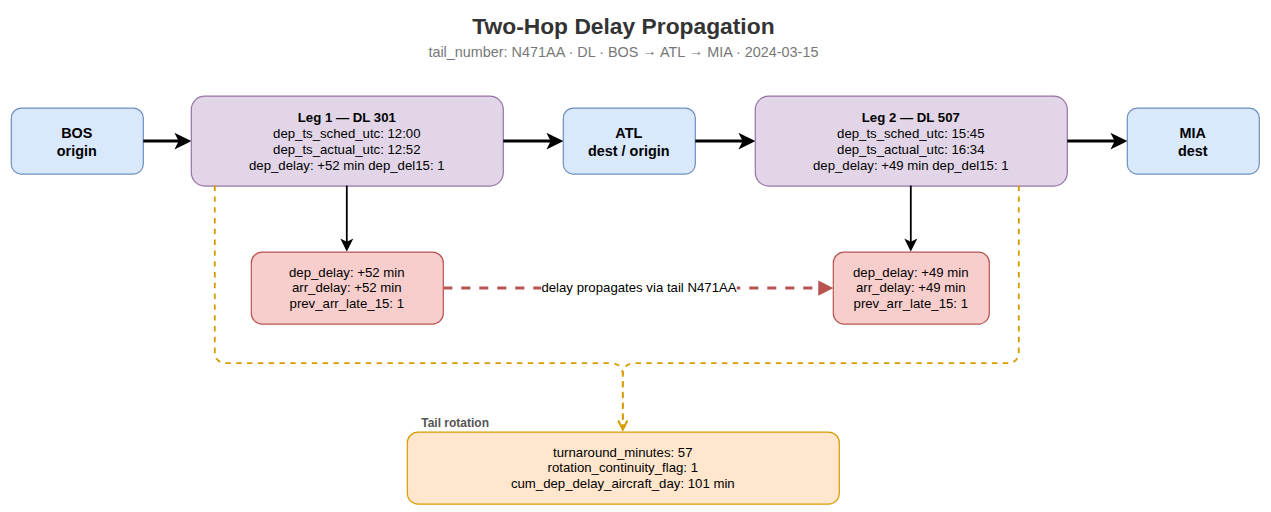
\includegraphics[width=1\linewidth,height=\textheight,keepaspectratio,alt={Diagram showing two flight legs sharing a tail number, with delay columns, weather as-of joins, and a propagation arrow connecting the delay on the first leg to the second.}]{images/paper/2-hop-prop.png}

}

\caption{\label{fig-two-hop}Two-hop delay propagation for tail N471AA
(BOS → ATL → MIA, 2024-03-15). A 52-minute departure delay on Leg 1
propagates to a 49-minute delay on Leg 2 via the tail rotation,
independent of weather conditions at the intermediate airport.}

\end{figure}%

Turnaround time captures the buffer between flights:

\[
Turnaround_i = DepartureTime_i - PreviousArrivalTime_i
\]

See Table~\ref{tbl-predictors} for more information on engineered
features.

\subsubsection{Postprocessing and
output}\label{postprocessing-and-output}

A \texttt{PostProcessConfig} object specifies the column subset retained
for modelling, allowing the full engineered dataset to be filtered to
task-specific representations without rerunning upstream stages. Final
outputs are written as monthly and annual Parquet files containing the
joined flight-weather records, alongside separate Parquet tables for the
canonical flight records, airport-time aggregates, route-time
aggregates, aircraft rotation sequences, and delay propagation chains.

\section{Prediction Targets}\label{prediction-targets}

We considered flight delay prediction as both a regression and
classification problem. Let

\[
Y_i^{(reg)} = \text{ArrDelay}_i
\]

denote the arrival delay in minutes for flight \(i\), and let

\[
Y_i^{(cls)} =
\begin{cases}
1 & \text{if } \text{ArrDel15}_i = 1 \\
0 & \text{otherwise}
\end{cases}
\]

denote whether the flight arrived at least 15 minutes late.

Thus, our predictive tasks were:

\begin{enumerate}
\def\labelenumi{\arabic{enumi}.}
\tightlist
\item
  \textbf{Regression:} predict continuous arrival delay in minutes.
\item
  \textbf{Classification:} predict whether a flight experiences a
  material arrival delay.
\end{enumerate}

\subsection{Raw Predictors and Important Data
Elements}\label{raw-predictors-and-important-data-elements}

Table Table~\ref{tbl-predictors} summarizes the major predictors and
supporting data elements used in the pipeline.

\begin{longtable}[]{@{}
  >{\raggedright\arraybackslash}p{(\linewidth - 4\tabcolsep) * \real{0.3333}}
  >{\raggedright\arraybackslash}p{(\linewidth - 4\tabcolsep) * \real{0.3333}}
  >{\raggedright\arraybackslash}p{(\linewidth - 4\tabcolsep) * \real{0.3333}}@{}}
\caption{Major predictors and important data items used in the flight
delay pipeline.}\label{tbl-predictors}\tabularnewline
\toprule\noalign{}
\begin{minipage}[b]{\linewidth}\raggedright
Category
\end{minipage} & \begin{minipage}[b]{\linewidth}\raggedright
Variables / Data Items
\end{minipage} & \begin{minipage}[b]{\linewidth}\raggedright
Description and Role in Modeling
\end{minipage} \\
\midrule\noalign{}
\endfirsthead
\toprule\noalign{}
\begin{minipage}[b]{\linewidth}\raggedright
Category
\end{minipage} & \begin{minipage}[b]{\linewidth}\raggedright
Variables / Data Items
\end{minipage} & \begin{minipage}[b]{\linewidth}\raggedright
Description and Role in Modeling
\end{minipage} \\
\midrule\noalign{}
\endhead
\bottomrule\noalign{}
\endlastfoot
Flight identifiers and route & \texttt{FlightDate},
\texttt{Reporting\_Airline}, \texttt{Tail\_Number}, \texttt{Origin},
\texttt{Dest}, \texttt{route\_key}, \texttt{flight\_id} & Core
identifiers used to define each flight, link feature tables, and
represent route-level context. \\
Schedule and realized timing & \texttt{CRSDepTime}, \texttt{DepTime},
\texttt{CRSArrTime}, \texttt{ArrTime}, \texttt{dep\_ts\_sched},
\texttt{dep\_ts\_actual}, \texttt{arr\_ts\_sched},
\texttt{arr\_ts\_actual}, UTC timestamp variants & Used to represent
schedule adherence, construct valid temporal ordering, and support
weather joins and aircraft rotation logic. \\
Delay targets and related operational outcomes & \texttt{ArrDelay},
\texttt{ArrDel15}, \texttt{DepDelay}, \texttt{DepDel15},
\texttt{Cancelled}, \texttt{Diverted} & Primary response variables and
closely related operational outputs used in modeling and filtering. \\
Surface movement and flight characteristics & \texttt{TaxiOut},
\texttt{TaxiIn}, \texttt{Distance}, \texttt{ActualElapsedTime} & Capture
operational complexity, congestion effects, and route structure. \\
Delay cause information & \texttt{CarrierDelay}, \texttt{WeatherDelay},
\texttt{NASDelay}, \texttt{LateAircraftDelay} & Useful for descriptive
analysis, route aggregation, and interpretation of operational drivers
of delay. \\
Temporal features & Departure hour, weekday, month, local date, UTC
date, seasonal indicators, holiday indicators & Capture cyclic demand,
seasonal traffic patterns, and calendar effects. \\
Airport reference data & Airport name, municipality, country, latitude,
longitude, IATA code, ICAO code, airport timezone & Used to map BTS
airports to weather stations, assign time zones, and support timestamp
normalization. \\
Weather station reference data & NOAA station ID, station timezone,
airport-to-station mapping & Used to associate flights with nearby
weather observations and enable correct UTC conversion of NOAA
timestamps. \\
Weather predictors & \texttt{dep\_temp\_c},
\texttt{dep\_wind\_speed\_m\_s}, \texttt{dep\_wind\_dir\_deg},
\texttt{dep\_ceiling\_height\_m}, \texttt{arr\_temp\_c},
\texttt{arr\_wind\_speed\_m\_s}, \texttt{arr\_wind\_dir\_deg},
\texttt{arr\_ceiling\_height\_m} & Represent meteorological conditions
associated with the departure and arrival environments. These are joined
temporally using the most recent prior observation within a two-hour
window. \\
Aircraft rotation / propagation features & Previous flight ID, previous
origin and destination, previous arrival delay, previous departure
delay, turnaround time, continuity flag, aircraft leg number, cumulative
delay by aircraft-day & Capture propagation effects caused by late
inbound aircraft and tight turnarounds. These were among the most
meaningful operational predictors. \\
Chain and cascade indicators & \texttt{has\_prev\_leg},
\texttt{has\_next\_leg}, \texttt{is\_middle\_leg}, tight turnaround
flags & Represent whether a flight is embedded within a larger aircraft
sequence and whether it is vulnerable to upstream or downstream delay
propagation. \\
Airport-time aggregate context & Hourly airport flight counts, average
delay, median delay, delay rate, cancellation rate, diversion rate, taxi
metrics, rolling means over 1h/3h/6h & Capture airport congestion and
short-horizon system state. \\
Route-time aggregate context & Hourly route counts, mean route delay,
route delay rate, average weather, rolling means over 1h/3h/6h & Capture
recent route-specific operating conditions and network-level delay
tendencies. \\
\end{longtable}

\subsection{Limitations in Data}\label{limitations-in-data}

Several limitations should be noted:

\begin{itemize}
\tightlist
\item
  BTS delay categories are aggregated and sometimes coarse
\item
  weather observations may not perfectly represent local flight
  conditions
\item
  route-level analysis cannot capture all national network effects
\item
  airline operational decisions such as crew scheduling are not directly
  observed
\end{itemize}

Despite these limitations, the dataset provides a strong foundation for
studying delay patterns.

\begin{itemize}
\tightlist
\item
  Add catalog as appendix item
\end{itemize}

\textbf{Note: create a section of the site that represents reproducable
instructions of our project and data processing steps, including code
snippets and explanations.}

\subsection{Initially started with a BWI--EWR Market
Pair}\label{initially-started-with-a-bwiewr-market-pair}

The BWI--EWR corridor sits within one of the most operationally complex
airspaces in the United States. Newark Liberty International Airport
operates within the highly congested New York airspace, while BWI serves
as a key mid-Atlantic hub.

Flights between these airports are vulnerable to multiple sources of
disruption:

\begin{itemize}
\tightlist
\item
  upstream aircraft delays
\item
  weather disruptions
\item
  airspace congestion
\item
  operational scheduling constraints
\end{itemize}

\section{EDA}\label{eda}

\begin{itemize}
\tightlist
\item
  Show network map of airports and flight routes - some kind of data
  visualization that shows the network structure of the flights between
  BWI and EWR, as well as other connecting routes. This could be a graph
  or a map visualization that highlights the frequency of flights and
  the connections between different airports.
\end{itemize}

\section{Feature Engineering}\label{feature-engineering-1}

\subsection{Delay Indicator}\label{delay-indicator}

\subsection{Prior Aircraft Delay}\label{prior-aircraft-delay}

\subsection{Temporal Features}\label{temporal-features}

Time-based indicators include:

\begin{itemize}
\tightlist
\item
  departure hour
\item
  day of week
\item
  month
\item
  holiday flags
\end{itemize}

These help capture cyclical delay patterns.

\begin{center}\rule{0.5\linewidth}{0.5pt}\end{center}

\section{Exploratory Data Analysis}\label{exploratory-data-analysis}

\subsection{Distribution of Delays}\label{distribution-of-delays}

\begin{Shaded}
\begin{Highlighting}[]
\CommentTok{\# Histogram of departure delays}
\CommentTok{\# ggplot(df, aes(x = DepDelayMinutes)) +}
\CommentTok{\#   geom\_histogram(bins = 50)}
\end{Highlighting}
\end{Shaded}

\subsection{Delays by Time of Day}\label{delays-by-time-of-day}

\begin{Shaded}
\begin{Highlighting}[]
\CommentTok{\# Delay frequency by departure hour}
\end{Highlighting}
\end{Shaded}

\subsection{Weather vs Delay}\label{weather-vs-delay}

\begin{Shaded}
\begin{Highlighting}[]
\CommentTok{\# Weather severity vs delay outcome}
\end{Highlighting}
\end{Shaded}

\subsection{Delay Propagation}\label{delay-propagation}

\begin{Shaded}
\begin{Highlighting}[]
\CommentTok{\# Previous arrival delay vs next departure delay}
\end{Highlighting}
\end{Shaded}

\begin{center}\rule{0.5\linewidth}{0.5pt}\end{center}

\begin{center}\rule{0.5\linewidth}{0.5pt}\end{center}

\section{Building Classifiers}\label{building-classifiers}

\subsection{Logistic Regression}\label{logistic-regression}

We begin with a baseline logistic regression model.

\[
P(Y_i = 1|X_i) =
\frac{1}{1 + e^{-\eta_i}}
\]

\[
\eta_i = \beta_0 + \beta_1 X_1 + \beta_2 X_2 + ... + \beta_p X_p
\]

\begin{Shaded}
\begin{Highlighting}[]
\CommentTok{\# logistic regression model}
\end{Highlighting}
\end{Shaded}

\begin{center}\rule{0.5\linewidth}{0.5pt}\end{center}

\subsection{Ridge Logistic Regression}\label{ridge-logistic-regression}

To address multicollinearity and improve stability we apply ridge
regularization.

\begin{Shaded}
\begin{Highlighting}[]
\CommentTok{\# ridge logistic regression}
\end{Highlighting}
\end{Shaded}

\begin{center}\rule{0.5\linewidth}{0.5pt}\end{center}

\subsection{Classification Tree}\label{classification-tree}

Decision trees provide interpretable classification rules.

\begin{Shaded}
\begin{Highlighting}[]
\CommentTok{\# classification tree}
\end{Highlighting}
\end{Shaded}

\begin{center}\rule{0.5\linewidth}{0.5pt}\end{center}

\subsection{Random Forest}\label{random-forest}

Random forests improve predictive accuracy through ensemble learning.

\begin{Shaded}
\begin{Highlighting}[]
\CommentTok{\# random forest model}
\end{Highlighting}
\end{Shaded}

\begin{center}\rule{0.5\linewidth}{0.5pt}\end{center}

\subsection{K-Nearest Neighbors}\label{k-nearest-neighbors}

KNN classifies flights based on nearby observations in feature space.

\begin{Shaded}
\begin{Highlighting}[]
\CommentTok{\# knn model}
\end{Highlighting}
\end{Shaded}

\begin{center}\rule{0.5\linewidth}{0.5pt}\end{center}

\section{Unsupervised Analysis}\label{unsupervised-analysis}

\subsection{Principal Component
Analysis}\label{principal-component-analysis}

PCA identifies dominant dimensions in the feature space.

\begin{Shaded}
\begin{Highlighting}[]
\CommentTok{\# PCA analysis}
\end{Highlighting}
\end{Shaded}

\subsection{K-Means Clustering}\label{k-means-clustering}

Clustering reveals natural groupings among flight observations.

\begin{Shaded}
\begin{Highlighting}[]
\CommentTok{\# kmeans clustering}
\end{Highlighting}
\end{Shaded}

\begin{center}\rule{0.5\linewidth}{0.5pt}\end{center}

\section{Model Comparison}\label{model-comparison}

We compare models using metrics such as:

\begin{itemize}
\tightlist
\item
  accuracy
\item
  precision
\item
  recall
\item
  F1 score
\end{itemize}

\begin{Shaded}
\begin{Highlighting}[]
\CommentTok{\# model comparison table}
\end{Highlighting}
\end{Shaded}

\begin{center}\rule{0.5\linewidth}{0.5pt}\end{center}

\section{Results}\label{results}

\subsection{Key Findings}\label{key-findings}

The analysis suggests that delay outcomes are influenced by several
interacting factors:

\begin{itemize}
\tightlist
\item
  upstream aircraft delays
\item
  airport congestion patterns
\item
  weather conditions
\item
  temporal scheduling effects
\end{itemize}

\subsection{Operational
Interpretation}\label{operational-interpretation}

Predictive models can help identify flights at elevated risk of delay
before departure, enabling airlines and planners to anticipate
disruptions.

\begin{center}\rule{0.5\linewidth}{0.5pt}\end{center}

\section{Discussion \& Limitations}\label{discussion-limitations}

Several limitations should be considered:

\begin{itemize}
\tightlist
\item
  missing operational factors such as crew and maintenance constraints
\item
  imperfect weather measurements
\item
  route-specific findings that may not generalize
\end{itemize}

Despite these challenges, the framework provides a replicable approach
for studying delay behavior.

\begin{center}\rule{0.5\linewidth}{0.5pt}\end{center}

\section{Conclusion}\label{conclusion}

This study demonstrates how machine learning methods can be applied to
understand delay dynamics in the BWI--EWR market pair.

Tree-based methods and penalized regression provide the best balance of
predictive performance and interpretability. The analysis highlights the
importance of upstream delay propagation and temporal operational
patterns.

Future work could extend this framework to larger airline networks and
incorporate time-series modeling approaches.

\begin{center}\rule{0.5\linewidth}{0.5pt}\end{center}

\section{References}\label{references}

\section{Appendix}\label{appendix}

\subsection{Data Catalog}\label{data-catalog}

\section{Hardware}\label{hardware}

The models were trained on a high-performance local workstation running
Ubuntu 22.04.5 LTS (64-bit) with kernel version 6.8. The system is
equipped with an AMD Ryzen 9 7900X processor featuring 24 logical cores
and boost speeds up to 5.65 GHz, along with approximately 96 GB of
system memory. The machine also includes both integrated AMD graphics
and a discrete NVIDIA GPU, although model training was conducted using
CPU resources. This hardware configuration provides substantial parallel
processing capability and memory bandwidth, enabling efficient handling
of large-scale data processing, feature engineering, and machine
learning model training workflows.

\section{Models}\label{models}

We are interested in building an multi-output model that both classifies
an arrival delay and determins how long that arrival delay will be using
features that are available during the present time.

Models: LSTM -

Model Arch units1 is the number of hidden units (neurons) in that LSTM
layer Each unit produces one value in the hidden state vector at each
time step. each neuron learns a pattern or signal from your inputs over
time. More units → more capacity → can learn more complex patterns Fewer
units → simpler model → less risk of overfitting

Break data into a step matrix - each example is broken into ordered
steps in time or sequence, rather than treated as one flat row. The LSTM
model needs this 3D matrix to work on. We apply some scaling to the data
to standardize each feature this allows our neural network to train more
effectively thus improving stability and convergence.

Flights contexts in 2 hop would be 3 different time steps. t-2, t-1, t0.
One sample would be 3 rows.

Varients - Use same training function but different inputs and model
sizes.

Making the model bigger adds more context: Answers Does adding richer
operational context improve sequence-based delay prediction?

By keeping the layers to only 2 hops we prevent the exploding gradient
problem To prevent the vanishing gradient problem we\ldots.else we would
never reach our optimal value LSTMs help us avoid the vanishing and
exploding gradient problems by using two seperate paths that are for
long and short term memories. The gates helps us make relavant
predictions only remmebering what is needed and forgetting what is not.
(explain)

Regularlization - We applied a dropout regularization to the LSTM
outputs, randomly turning off a fraction (dropout, e.g., 20\%) of the
neurons during training. This helps prevent the model from overfitting
by forcing it to not rely too heavily on any single pattern or feature.

Loss Functions Binary Cross-Entroy

\[
\mathcal{L}_{BCE} = -\frac{1}{N} \sum_{i=1}^{N} \left[ y_i \log(p_i) + (1 - y_i) \log(1 - p_i) \right]
\]

MSE \[
\mathcal{L}_{MSE} = \frac{1}{N} \sum_{i=1}^{N} (y_i - \hat{y}_i)^2
\]

Evaluation Metrics

Cross Validation and Hyper Parameter Tuning

Train-Test Splits for CV. Expanding window folds inside Jan-Oct training
period.

\begin{verbatim}
Fold 1: train Jan-Jun, validate Jul
Fold 2: train Jan-Jul, validate Aug
Fold 3: train Jan-Aug, validate Sep
Fold 4: train Jan-Sep, validate Oct
\end{verbatim}

FINAL TEST SPLIT \# Keep Nov-Dec untouched

Tree -

Metrics: Classification - AUC, F1, precision, recall, accuracy\\
Regression - MAE, RMSE

\begin{itemize}
\tightlist
\item
  Explain why used and are there better ones to use
\end{itemize}

Rows in final modeling table: 6594553 Train rows: 5490189 (Jan 1-Oct 31)
Test rows : 1104364 (Nov 1-Dec 31)

The code performs a time-based train/test split on the flights dataset
using November 1, 2019 as the cutoff. A temporal split like this is the
correct approach for LSTM modeling on time-series data, as it mirrors
real-world prediction conditions and prevents data leakage from future
records into training.it is important to split your training and test
sets by a fixed date rather than randomly. Random splitting allows
future data to leak into the training set, meaning the model
inadvertently learns from information it would not have had access to in
a real-world scenario. By splitting on a specific date like November 1,
2019, we ensure the model is only trained on the past and evaluated on
truly unseen future data, which gives a more honest and reliable measure
of model performance.

\begin{itemize}
\tightlist
\item
  Add diagram of model training and evaluation process - move to
  modeling section
\end{itemize}

\protect\phantomsection\label{refs}
\begin{CSLReferences}{0}{0}
\bibitem[\citeproctext]{ref-bts_ontime}
\CSLLeftMargin{{[}1{]} }%
\CSLRightInline{Bureau of Transportation Statistics, {``Airline on-time
performance data.''} \url{https://transtats.bts.gov/}; U.S. Department
of Transportation, 2025.}

\bibitem[\citeproctext]{ref-noaa_ncei}
\CSLLeftMargin{{[}2{]} }%
\CSLRightInline{National Oceanic and Atmospheric Administration, {``NCEI
global hourly weather dataset.''}
\url{https://www.ncei.noaa.gov/access/services/data/v1}; NOAA National
Centers for Environmental Information, 2025.}

\bibitem[\citeproctext]{ref-noaa_isd_history}
\CSLLeftMargin{{[}3{]} }%
\CSLRightInline{National Oceanic and Atmospheric Administration,
{``Integrated surface database (ISD) station history.''}
\url{https://www.ncei.noaa.gov/pub/data/noaa/isd-history.csv}; NOAA,
2025.}

\bibitem[\citeproctext]{ref-ourairports}
\CSLLeftMargin{{[}4{]} }%
\CSLRightInline{OurAirports, {``OurAirports global airport database.''}
\url{https://davidmegginson.github.io/ourairports-data/airports.csv};
OurAirports, 2025.}

\end{CSLReferences}




\end{document}
